\documentclass[
	aspectratio=169, % default is 43
	8pt, % font size, default is 11pt
	%handout, % < do not remove this comment, it is used by the Makefile >
]{beamer}
\def\university{} % < do not remove this comment, it is used by the Makefile >

\documentclass[
	aspectratio=169, % default is 43
	8pt, % font size, default is 11pt
	handout, % handout mode without animations, comment out to add animations
]{beamer}

\usepackage{../template/beamerthemeuulm} % use the inofficial uulm beamer theme
\setfaculty{infIngPsy} % set the color scheme for your faculty here [med/infIngPsy/math/nat]

% requires symbolic links
% git clone git@github.com:SoftVarE-Group/SlideTemplate.git C:\Users\...\SlideTemplate
% mklink /J template C:\Users\...\SlideTemplate
% git clone git@spgit.informatik.uni-ulm.de:thuem/slides.git C:\Users\...\ThomasSlides
% mklink /J thomasslides C:\Users\...\ThomasSlides
\graphicspath{{../template/pics/logos}{../template/pics/nature}{../template/pics/uulm}{../thomasslides/}{../pics/people/}{../pics/xkcd/}}

%\usepackage[ngerman]{babel} % use this line for slides in German
%\recordingtrue % special recording mode for use with a greenscreen, gives you space to show yourself in a layer in front of the slides, has no effect in the handout mode

\title{Software Product Lines} % short title is used for the slide footer but optional

% LINKED LITERATURE

\newcommand{\ludewiglichter}{\href{https://learning.oreilly.com/library/view/-/9781457184932/?ar}{Ludewig and Lichter}}
\newcommand{\seeconomics}{\href{https://rds-ulm.ibs-bw.de/link?kid=027381854}{SE Economics}}
\newcommand{\sommervillelink}[1]{\href{https://ulm.ibs-bw.de/aDISWeb/app?service=direct/0/Home/$DirectLink\&sp=SOPAC00\&sp=SAKSWB-IdNr1615420983}{#1}}
\newcommand{\sommerville}{\sommervillelink{Sommerville}}
\newcommand{\thehumbleprogrammer}{\href{https://dl.acm.org/doi/10.1145/1283920.1283927}{The Humble Programmer}}
\newcommand{\thepragmaticprogrammer}{\href{https://learning.oreilly.com/library/view/the-pragmatic-programmer/9780135956977/}{The Pragmatic Programmer}}

% TYPICAL COMMANDS FOR LECTURES

\renewcommand{\emph}[1]{{\color{blue}\textbf{#1}}}

\newcommand{\deutsch}[1]{{\color{blue}(#1)}}
\newcommand{\deutschertitel}[1]{{\tiny\deutsch{#1}}}

\newcommand{\mycite}[1]{``#1''}
\newcommand{\mytitlesource}[1]{{\tiny\normalfont\mbox{[#1]}}}
\newcommand{\mysource}[1]{\ifthenelse{\equal{#1}{}}{}{\phantom{.}~\hfill~\mytitlesource{#1}}}

\newcommand{\todo}[1]{{\color{red}\textbf{[#1]}}}
\newcommand{\fodo}[1]{\todo{\footnote{\todo{#1}}}}
\newcommand{\todots}{\todo{\ldots}}

% IMPORTED PACKAGES

%\usepackage{adjustbox} % used for partofpage
%\usepackage{tcolorbox} % used for mydefinition, mynote, myexample
\usepackage{multicol} % used temporarily for the lecture overview
\usepackage{mathtools} % required for absolute value in modeling lecture

% COMMANDS TO LAYOUT AND ANNIMATE SLIDES

\newcommand{\lessonslearned}[3]{
	\subsection{Summary}
	\begin{frame}{\insertsection -- \insertsubsection}
		\leftorright{
			\mydefinition{Lessons Learned}{
				\begin{itemize}
					#1
				\end{itemize}
			}
			\mynote{Further Reading}{
				\small % references take space, can be a little smaller
				\begin{itemize}
					#2
				\end{itemize}
			}
		}{
			\myexample{Practice}{
				#3
			}
		}
	\end{frame}
}

% TODO temporary hack to layout the slide overview in two colums
\renewcommand{\lectureoverview}{
%	\section*{Overview}
%	\subsection*{Overview}
	\begin{frame}{\insertsubtitle}
		\begin{multicols}{2}
			\tableofcontents
		\end{multicols}
	\end{frame}
}

\renewcommandx{\maketitle}[2][1=apr21-o25a,2=150]{
    {
	\usebackgroundtemplate{} % TODO temporary hack to enable missing pictures at title slide
	%\ifx {#1} \empty \else {\usebackgroundtemplate{\includegraphics[trim=0 0 0 #2,clip,width=\paperwidth]{#1}}} \fi     
	%\usebackgroundtemplate{\includegraphics[trim=0 0 0 #2,clip,width=\paperwidth]{#1}}
    \begin{frame}[plain]
        \vskip0pt plus 1filll
        \begin{beamercolorbox}[wd=\paperwidth,ht=4.5ex,dp=2ex,right]{titlebox}
            \LARGE\textbf{\inserttitle}\hspace*{20pt}
        \end{beamercolorbox}%
        \nointerlineskip%
        \begin{beamercolorbox}[wd=\paperwidth,ht=2.25ex,dp=1ex,right]{subtitlebox}
            \small 
            \ifx \insertsubtitle \empty \else \insertsubtitle\ $\vert$ \fi
            \insertauthor\
            \ifx \insertdate \empty \else $\vert$ \insertdate \fi
            \hspace*{20pt}
        \end{beamercolorbox}%
        \nointerlineskip%
        \begin{beamercolorbox}[wd=\paperwidth,ht=4.5ex,dp=2ex,left]{logobox}
            \centering
            \vspace{-1ex}
            \hspace{10pt}
            \includegraphics[height=4.5ex]{sp} % SPECIFY INSTITUTE LOGO HERE
            \hfill
            \includegraphics[height=4.5ex]{uulm}
            \hspace{10pt}
        \end{beamercolorbox}%
    \end{frame}
    }  
}

%
%\newcommand{\onlyleft}[1]{
%	\halfpage{#1}
%}
%
%\newcommand{\onlyright}[1]{
%	~\hfill
%	\halfpage{#1}
%}
%
%\newcommand{\leftorright}[2]{
%	\uncover<1>{\halfpage{#1}}
%	\hfill
%	\uncover<3->{\halfpage{#2}}
%}
%
%\newcommand{\rightorleft}[2]{
%	\uncover<3->{\halfpage{#1}}
%	\hfill
%	\uncover<1>{\halfpage{#2}}
%}
%
%\newcommand{\leftthenright}[2]{
%	\halfpage{#1}
%	\hfill\pause
%	\halfpage{#2}
%}
%
%\newcommand{\leftandright}[2]{
%	\halfpage{#1}
%	\hfill
%	\halfpage{#2}
%}
%
%\newcommand{\leftmiddleandright}[3]{
%	\thirdpage{#1}
%	\hfill
%	\thirdpage{#2}
%	\hfill
%	\thirdpage{#3}
%}
%
%\newcommand{\leftmiddleorright}[3]{
%	\uncover<1>{\thirdpage{#1}}
%	\hfill
%	\uncover<3>{\thirdpage{#2}}
%	\hfill
%	\uncover<5->{\thirdpage{#3}}
%}
%
%\newcommand{\halfpage}[1]{\partofpage{48}{#1}}
%
%\newcommand{\thirdpage}[1]{\partofpage{31}{#1}}
%
%\newcommand{\partofpage}[2]{
%	\adjustbox{valign=t}{\begin{minipage}{0.#1\textwidth}
%			\begin{flushleft}
%				#2
%			\end{flushleft}
%	\end{minipage}}
%}
%
%\newcommand{\mydefinition}[2]{
%	\begin{tcolorbox}[title=#1,colback=orange!10,colframe=orange!30,coltitle=black,fonttitle=\bfseries,left=1mm,right=1mm,top=1mm,bottom=1mm]
%		\begin{flushleft}
%			#2
%		\end{flushleft}
%	\end{tcolorbox}
%}
%
%\newcommand{\mydefinitiontight}[2]{
%	\begin{tcolorbox}[title=#1,colback=white,colframe=orange!30,coltitle=black,fonttitle=\bfseries,left=0mm,right=0mm,top=0mm,bottom=0mm]
%		\begin{flushleft}
%			#2
%		\end{flushleft}
%	\end{tcolorbox}
%}
%
%\newcommand{\mynote}[2]{
%	\begin{tcolorbox}[title=#1,colback=red!10,colframe=red!30,coltitle=black,fonttitle=\bfseries,left=1mm,right=1mm,top=1mm,bottom=1mm]
%		\begin{flushleft}
%			#2
%		\end{flushleft}
%	\end{tcolorbox}
%}
%
%\newcommand{\myexample}[2]{
%	\begin{tcolorbox}[title=#1,colback=blue!10,colframe=blue!30,coltitle=black,fonttitle=\bfseries,left=1mm,right=1mm,top=1mm,bottom=1mm]
%		\begin{flushleft}
%			#2
%		\end{flushleft}
%	\end{tcolorbox}
%}
%
%\newcommand{\myexampletight}[2]{
%	\begin{tcolorbox}[title=#1,colback=white,colframe=blue!30,coltitle=black,fonttitle=\bfseries,left=0mm,right=0mm,top=0mm,bottom=0mm]
%		\begin{flushleft}
%			#2
%		\end{flushleft}
%	\end{tcolorbox}
%}

\subtitle{1. Introduction}
\author{Thomas Thüm, Timo Kehrer, Elias Kuiter}
\ifuniversity{magdeburg}{\setpicture[70]{ovgu-autumn1}\setcopyright{Photo: Hannah Theile (OVGU)}}

\begin{document}

\mode<handout>{\contentoverview}

\mode<beamer>{
	\ifdefined\thepicture
		\maketitle[\thepicture][\thepictureoffset]
	\else
		\maketitle[]
	\fi
}

% shared slide content

% introduced: 02a-configuration
% reused: 03a-intro
\newcommand{\frameImplementSPLs}{
	\begin{mycolumns}[widths={45},animation=none]
		\pic[width=\linewidth]{metaproduct2}
	\mynextcolumn
		\begin{note}{Key Issues}
			\begin{itemize}
			\item Systematic reuse of implementation artifacts
			\item Explicit handling of variability
			\end{itemize}
		\end{note}
		\uncover<2->{\begin{definition}{Variability\mysource{\fospl\mypage{48}}}
			\mycite{\emph{Variability} is the ability to derive different products from a common set of artifacts.}
		\end{definition}}
		~
		\uncover<3->{\begin{note}{Variability-Intensive System}
			Any software product line is a variability-intensive system. % TODO Timo: do we really need this term? where does this definition come from?
		\end{note}}
	\end{mycolumns}
}

% introduced: 02a-configuration
% reused: 02b-implementation, 03a-intro
\newcommand{\frameVariabilityAndBindingTimes}{
	\begin{mycolumns}[widths={55},animation=none]
		\begin{definition}{Binding Time \deutsch{Bindungszeitpunkt}\mysource{\fospl\mypage{48}}}
			\begin{itemize}
				\item Variability offers choices
				\item Derivation of a product requires to make decisions (aka. binding)
				\item Decisions may be bound at different binding times
			\end{itemize}
		\end{definition}
		~
		\uncover<2->{\begin{note}{When? By whom? How?}
			\lectureruntime\parta: \emph{when} and \emph{by whom}

			\lectureruntime\partb: \emph{how}
		\end{note}}
	\mynextcolumn
		\pic[width=\linewidth]{metaproduct2}
	\end{mycolumns}
}

% introduced: 03a-intro
% reused: 03a-intro
\newcommand{\frameRuntimeVariabilityProblems}{
	\begin{note}{Problems of Runtime Variability}
		{\bf Conditional Statements:}
		\begin{itemize}
			\item Code scattering, tangling, and replication
		\end{itemize}
		{\bf Design Patterns for Variability:}
		\begin{itemize}
			\item Trade-offs and potential negative side effects
			\item Constraints that may restrict their usage
		\end{itemize}
		{\bf In General:}
		\begin{itemize}
			\item Variable parts are always delivered
			\item Not well-suited for compile-time binding
		\end{itemize}
	\end{note}
}

% introduced: 03a-intro
% reused: 03a-intro
\newcommand{\frameSoftwareConfigurationManagement}{
	\begin{mycolumns}
		\begin{definition}{Software Configuration Management} % TODO source missing
			Policies, processes, and tools for managing evolving software systems:
			\begin{itemize}
				\item Version control
				\item System building
				\item Release management
				\item Change management
				\item Collaborative work
			\end{itemize}
		\end{definition}
	\mynextcolumn
		\begin{note}{No Software Configuration Management}
			\lecturecloneandown\parta: Ad-Hoc Clone-and-Own

			aka.\ unmanaged clone-and-own
		\end{note}
		\begin{note}{Version Control}
			\lecturecloneandown\partb: Clone-and-Own with Version Control

			instance of managed clone-and-own
		\end{note}
		\begin{note}{System Building}
			\lecturecloneandown\partc: Clone-and-Own with Build Systems

			instance of managed clone-and-own
		\end{note}
	\end{mycolumns}
}


\section{Introduction to Product Lines}

\begin{frame}
	\ifuniversity{ulm}{for ulm}
	\ifuniversity{magdeburg}{for md}
\end{frame}

\subsection{Handcrafting and Customization}
\begin{frame}{What do these examples have in common?}
	\begin{mycolumns}[columns=3,widths={35,28},animation=none]
		\pic[width=\linewidth,trim=25 200 25 25,clip]{wedding}
		
		\pic[width=\linewidth]{shoes}
	\mynextcolumn
		\pic[width=\linewidth,trim=85 0 0 0]{eiffel-tower}
	\mynextcolumn
		\pic[width=\linewidth,trim=70 35 0 0]{draisine}
		
		~
		
		\uncover<2->{\begin{definition}{Customization \deutschertitel{Maßschneiderung}}
			\begin{itemize}
			\item aka.\ handcrafting
			\item labor-intensive production
			\item highly individual goods
			\end{itemize}
		\end{definition}}
	\end{mycolumns}
\end{frame}

\begin{frame}{Customization of Elevators}
	\begin{mycolumns}[columns=4,T]
		\centering\pic[width=\linewidth]{elevator1-out}

		two buttons
	\mynextcolumn
		\centering\pic[width=\linewidth]{elevator2-out2}

		one button
	\mynextcolumn
		\centering\pic[width=\linewidth]{elevator3-out}

		keyhole
	\mynextcolumn
		\centering\pic[width=\linewidth]{elevator2-out1}

		floor display
	\end{mycolumns}
\end{frame}

\begin{frame}{Customization of Elevators}
	\begin{mycolumns}[columns=4,widths={28,21,28,21},T]
		\centering\pic[width=\linewidth]{elevator1-in2}

		no button to close door
	\mynextcolumn
		\centering\pic[width=\linewidth]{elevator3-in1}

		two keyholes
	\mynextcolumn
		\centering\pic[width=\linewidth]{elevator4-in}

		keycard
	\mynextcolumn
		\centering\pic[width=\linewidth]{elevator2-in2}

		double tap for~undo
	\end{mycolumns}
\end{frame}

\subsection{Mass Production}
\begin{frame}[b]{\myframetitle}
	\vspace{-\textheightoftitle}
	\begin{mycolumns}[b]
		\begin{definition}{Mass Production \deutschertitel{Massenproduktion}\mysource{\fospl\mypages{3--4}}}
			\begin{itemize}
			\item consequence of industrialization
			\item goods are produced from standardized parts
			\item improved productivity wrt.\ handcrafting
			\item reduced costs, improved quality
			\item but: (almost) no individualism
			\end{itemize}
		\end{definition}
		\uncover<2->{\begin{example}{Principle: One Size Fits All}
			\begin{itemize}
			\item t-shirts: XS, S, M, L, XL, XXL
			\item swiss-army knife \deutsch{Eierlegende Wollmilchsau}
			\end{itemize}
		\end{example}
		\centering\pic[width=.45\linewidth]{wollmilchsau}}
	\mynextcolumn
		\pic[width=\linewidth]{swiss-army-knife}
		\uncover<3->{\begin{note}{Mass Production for Software?\mysource{\fospl\mypage{7}}}
			\mycite{The idea is to provide software that satisfies the needs of most customers, which leads almost automatically to the situation, in which customers miss desired functionality and are overwhelmed with functionality they do not need actually (just think of any contemporary office or graphics program). It is often this generality that makes software complex, slow, and buggy.}
		\end{note}}
	\end{mycolumns}
\end{frame}
% industrial revolution/era:
% - John Hall, exchangable parts 1826, 25 years of trials (source?)
% - Henry Ford/Ransom Olds, production/assembly line, 1901 (source?)
% - 1961 first industrial roboter at General Motors
% - 1980s automatic assembly lines

\subsection{Mass Customization}
\begin{frame}{About Every Second Car is Unique}
	\centering\pic[width=.66\linewidth]{many-cars}
\end{frame}
\begin{frame}{\myframetitle\ \deutschertitel{Kundenindividuelle Massenproduktion}}
	\begin{mycolumns}[widths={45}]
		\begin{definition}{Mass Customization\mysource{\fospl\mypage{4}}}
			\begin{itemize}
			\item = mass production + customization
			\item customized, individual goods at costs similar to mass production
			\end{itemize}
		\end{definition}
		\myexampletight{Car Configuration}{\pic[width=\linewidth]{toyota-aygo-wheels}}
	\mynextcolumn
		\myexampletight{Car Production}{\pic[width=\linewidth,trim=0 50 0 240,clip]{car-manufacturing}}
		\begin{example}{Other Domains}
			bikes, computers, electronics, tools, medicine, clothing, food, financial services, \ldots, software?
		\end{example}
	\end{mycolumns}
\end{frame}

\begin{frame}{Mass Customization for Software?}
	\begin{mycolumns}[b,widths={55},animation=none]
		\begin{definition}{Mass Customization for Software?}
			\begin{itemize}
			\item customization: individual software developed using Waterfall model or Scrum
			\item mass production: standard software developed once for millions or billions of users (e.g.,~Whatsapp messenger)
			\item mass customization: software product lines
			\end{itemize}
		\end{definition}
		\uncover<2->{\begin{note}{Why Software Product Lines?}
			\begin{itemize}
			\item resource limitations: memory, performance, energy
			\item different hardware
			\item different laws
			\item goal: avoid expensive customization
			\item how is software developed?
			\end{itemize}
		\end{note}}
	\mynextcolumn
		\pic[width=\linewidth,trim=250 0 0 0,clip]{car-tower}
	\end{mycolumns}
\end{frame}

\subsection{Recap: The Software Life Cycle}
\begin{frame}{The Project Cartoon}
	\renewcommand{\projectcartoonwidth}{.135}
	\uncover<2-|handout:1-2>{\alt<-8|handout:1>{\hprojectcartoon{01}{how the customer explained it}}{\alt<9|handout:2>{\hprojectcartoon{01}{Requirements}}{\projectcartoon{01}{Requirements}}}}% requirements
	\uncover<3->{\alt<-8,10-|handout:1>{\hprojectcartoon{02}{how the project leader understood it}}{\projectcartoon{02}{how the project leader understood it}}}% modeling
	\uncover<4->{\alt<-8,10-|handout:1>{\hprojectcartoon{03}{how the analyst designed it}}{\projectcartoon{03}{how the analyst designed it}}}% architecture and design
	\uncover<5->{\alt<-8,10-|handout:1>{\hprojectcartoon{04}{how the programmer implemented it}}{\projectcartoon{04}{how the programmer implemented it}}}% implementation
	\uncover<6->{\alt<-8,10-|handout:1>{\hprojectcartoon{05}{what the beta testers received}}{\projectcartoon{05}{what the beta testers received}}}% testing
	\uncover<7->{\alt<-8,10-|handout:1>{\hprojectcartoon{10}{how it was supported}}{\projectcartoon{10}{how it was supported}}}% maintenance
	\uncover<8->{\alt<-8|handout:1>{\hprojectcartoon{13}{what the customer really needed}}{\alt<9>{\hprojectcartoon{13}{Product}}{\projectcartoon{13}{Product}}}}% customer / SE II
	\\
\end{frame}

\begin{frame}{\myframetitle\ \deutschertitel{Software-Lebenszyklus}}
	\waterfallcartoon\\
\end{frame}

\subsection{Features and Products of a Domain}
\begin{frame}{What is a Feature?}
	\begin{mycolumns}[widths={45},t]
		\uncover<2->{\begin{definition}{Feature \deutsch{Feature} \mysource{\fospl\mypage{18}}}
			\mycite{A \emph{feature} is a characteristic or end-user-visible behavior of a software system.}
		\end{definition}}
		\centering\xkcd{2369}{width=.9\linewidth,trim=35 35 35 35,clip}
	\mynextcolumn
		\uncover<3->{\begin{note}{Feature in a Product Line \mysource{\fospl\mypage{18}}}
			\mycitebegin Features are used in product-line engineering
			\begin{itemize}
				\item to specify and communicate commonalities and differences of the products between stakeholders \deutsch{Akteure} and
				\item to guide structure, reuse, and variation across all phases of the software life cycle.\myciteend
			\end{itemize}
		\end{note}}
		\renewcommand{\projectcartoonwidth}{.18}\scriptsize
		\uncover<4->{\waterfallcartoon}\\
	\end{mycolumns}
\end{frame}
% TODO picture of a program highlighting one or two features? settings? changelog? marketing description of new features (Github?)?

% goals of features
%a distinctively identifiable functional abstraction that must be implemented, tested, delivered, and maintained” (Kang et al.
%a product characteristic from user or customer views, which essentially consists of a cohesive set of individual requirements” (Chen et al.
%an optional or incremental unit of Zave 2003) 

\begin{frame}{What is a Product?}
	\begin{mycolumns}[t,animation=none]
		\begin{definition}{Product \deutsch{Produkt} \mysource{\fospl\mypage{19}}}
			\mycite{A \emph{product of a product line} is specified by a valid feature selection (a subset of the features of the product line). A feature selection is \emph{valid} if and only if it fulfills all feature dependencies.}
		\end{definition}
		\uncover<2->{\begin{note}{Note on Terminology}
			\begin{itemize}
				\item in this course:\\product = product variant = variant
				\item software product: a product consisting only of software
				\item software is more than a program: requirements, models, source code, tests, documentation
				\item this course focuses on source code
			\end{itemize}
		\end{note}}
		% TODO exemplify difference between hardware product, software product (VLC?), and program (reuse pictures from before)
	\mynextcolumn
		\uncover<3->{\myexampletight{Product Map for Eclipse (excerpt)}{
			\pic[width=\linewidth,trim=0 460 635 0,clip]{eclipse-product-map}
		}}
	\end{mycolumns}
\end{frame}
% TODO Venn diagram could also be a good visualization: products correspond to sets and features to set elements

\begin{frame}{What is a Domain?}
	\begin{mycolumns}[animation=none]
		\begin{definition}{Domain \deutsch{Domäne} \mysource{\fospl\mypage{19}}} % TODO cite CE00 here too?
			\mycitebegin A \emph{domain} is an area of knowledge that:
			\begin{itemize}
				\item is scoped to maximize the satisfaction of the requirements of its stakeholders,
				\item includes a set of concepts and terminology understood by practitioners in that area,
				\item and includes the knowledge of how to build software systems (or parts of
				software systems) in that area.\myciteend
			\end{itemize}
		\end{definition}
		\uncover<2->{\begin{note}{Features of a Domain}
			\begin{itemize}
				\item a feature is a domain abstraction
				\item identification of features in a domain requires domain expertise
				\item later: select features for a product line?
			\end{itemize}
		\end{note}}
	\mynextcolumn
		\pic[width=.5\linewidth]{many-cars}

		\hfill\xkcd{2369}{width=.5\linewidth,trim=35 35 35 35,clip}\hfill{}

		\hfill\pic[width=.5\linewidth]{eclipse-luna}
	\end{mycolumns}
\end{frame}
% TODO add more examples for domains

\subsection{Software Product Line}
\begin{frame}{\myframetitle}
	\begin{mycolumns}[widths={78},columns=1]
		\begin{definition}{Software Product Line \mysource{\seiwhitepaperspl\mypage{5}}}
			\mycitebegin A \emph{software product line} is
			\begin{itemize}
				\item a set of software-intensive systems \uncover<2->{\myexampletight{}{aka.\ products or variants}}
				\item that share a common, managed set of features \uncover<3->{\myexampletight{}{common set, but not all products have all features in common}}
				\item satisfying the specific needs of a particular market segment or mission \uncover<4->{\myexampletight{}{aka.\ domain \deutsch{Domäne, Einsatzgebiet, Marktsegment}}}
				\item and that are developed from a common set of core assets in a prescribed way.\myciteend \uncover<5->{\myexampletight{}{aka.\ planned, structured reuse \deutsch{Wiederverwendung von vorbereiteten Teilen}}}
				\mysource{\href{https://resources.sei.cmu.edu/library/asset-view.cfm?assetID=513819}{Software Engineering Institute, Carnegie Mellon University}}
			\end{itemize}
		\end{definition}
	\end{mycolumns}
\end{frame}
% variants / platforms / domain / variant generation
% configurable software, highly-configurable software, variable software, software variation

\subsection{Product-Line Engineering}
\begin{frame}{\myframetitle}
	\begin{mycolumns}[animation=none]
		\begin{definition}{Product-Line Engineering\mysource{\sple\mypage{14}}}
			\mycite{\emph{Software product-line engineering} is a paradigm to develop software applications (software-intensive systems and software products) using software platforms and mass customization.}
%			\begin{itemize}
%			\item aka.\ product-line development \mysource{\seiwhitepaperspl\mypage{207}}
%			\end{itemize}
		\end{definition}
		\uncover<2->{\begin{note}{Promises of Product Lines \mysource{\fospl\mypages{9--10}}}
			\begin{itemize}
				\item tailor-made \deutsch{Maßschneiderung}
				\item reduced costs \deutsch{Kostenreduzierung}
				\item improved quality \deutsch{Qualitätssteigerung}
				\item reduced time-to-market \deutsch{Reduzierung der Produktentwicklungszeit}
			\end{itemize}
		\end{note}}
	\mynextcolumn
		\vspace{-5mm}
		\uncover<3->{\mynotetight{Idea of Product-Line Engineering}{
			Reduce effort per product by means of an up-front investment for the product line:
			
			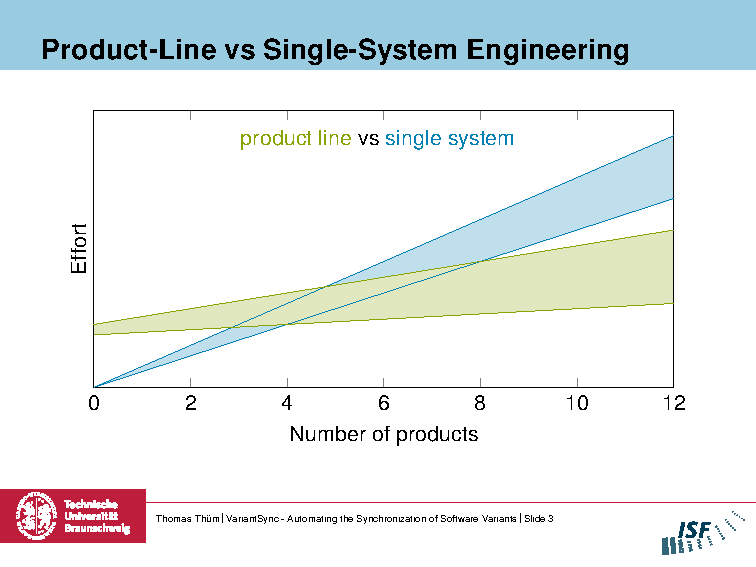
\includegraphics[width=\linewidth,trim=30 60 30 50,clip]{product-line-vs-single-system}
		}}
		\uncover<4->{\begin{definition}{Single-System Engineering}
			\begin{itemize}
			%\item aka.\ single-system development \mysource{\seiwhitepaperspl\mypage{7}}
			\item \deutsch{Einzelsystementwicklung}
			\item classical software development that is not considered as product-line engineering
			\end{itemize}
		\end{definition}}
	\end{mycolumns}
\end{frame}

% product-line hall of fame
% success stories: Boing, Bosch, Hewlett Packard, Toshiba, General Motors \mysource{\fospl}

% TODO \subsection{Running Examples?}
% \fospl: data management for embedded systems, product line of a graph library

% not software, not running: financial services (or in \lecturemodeling?), bikes, shoes, notebooks, ...
% Linux, Graph Product Line \lectureruntime\ or \lecturecloneandown, Configurable Database, Elevator Product Line, Printer product lines, Car configurators, software ecosystem (Browser plug-ins, IDE plug-ins)

% elevators: pictures from various elevators (OVGU, UULM, Bern), invisible end-user-visible features (e.g., double click for deselection)
% if you do this at home: do not select all stops before you know it is working

% how many examples in first lecture? move certain examples in later lectures? if so, which ones?
%\subsection{Automotive Systems}
% car configurators
% history? number of variants over time?
%\subsection{Notebooks}
% lenovo, microsoft, apple
%\subsection{Printer (Firmware)}
% real printers, 3d printers
% 30 printers per year, more examples
% XKCD: all-in-one paper processor
%\subsection{Operating Systems}
% windows, linux!!!, android
% Linux: where is it used? on which principal hardware? how many instances are running world wide? how many commits and developers? how many versions have been release and since when? screenshot how it looks like when linux is configured
% apps?
%\subsection{Integrated Development Environments}
% eclipse
%\subsection{Browsers}
% plug-ins

% apps! in market store android, iOS
% ecos, packages in debian

%\subsection{Beyond Software}
% financial products by KfW, bikes, shoes, muesli, Subway, headphones, lego, detergents, furniture (handcrafted vs standardized vs product line), kitchens
% brompton: picture in ulm slides

% zoo of animals/tools

% historical development? exchangable parts, production lines, automated product lines, ...
% all-in-one solution vs custom development? software for German fire departments
% all-in-one application software vs embedded software
% reasons for custom development: 

% goal of the lecture

%\subsection{Features}

%\subsection{Software Product Lines}
%% product-line engineering
%\begin{frame}{Who Produces Only One Product?}
%	\href{https://pxhere.com/en/photo/920906}{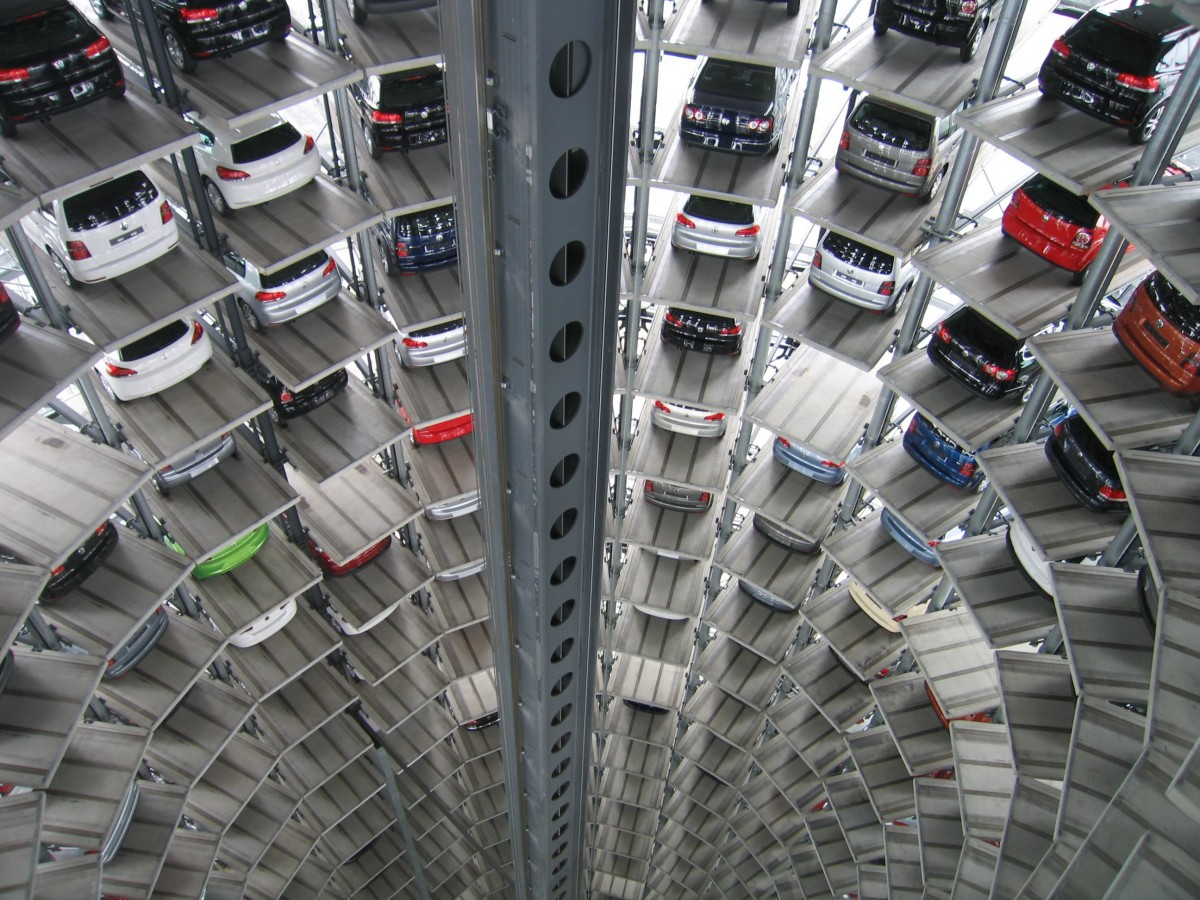
\includegraphics[width=.6\linewidth]{car-tower}}
%\end{frame}

%\subsection{Single System}
%% single-system engineering
%
%\begin{frame}{Greenfield Development? \deutschertitel{Auf der grünen Wiese?}}
%	\href{https://github.com/SoftVarE-Group/SlideTemplate/blob/main/pics/nature/may21-ulm.jpg}{\includegraphics[width=.6\linewidth]{may21-ulm}}
%\end{frame}



% add illustration for variants/versions (space/time) by icons of word/excel/powerpoint/one note/... over the years




% Apel 2013, Page 49
%Compile-time variability is decided before or at compile time.
%Load-time variability is decided after compilation when the program is started.
%With run-time variability, decisions can be made and changed during program
%execution.



% explain configurators vs selectors? for example, iPhone is available is produced in any combination and then selled, still there are selectors to find the right product easily. cf. ebay/amazon




% history on product lines? how old are product lines and ideas discussed in this lecture?






\lessonslearned{
	\item mass customization = mass production + customization
	\item features, products, domains
	\item software product lines
	\item product-line engineering
}{
	\item[] \fospl, Chapter~1\mypages{3--15}
}{
	\begin{itemize}
		\item What other examples of product lines do you know?
		\item Exemplify the differences between feature, product, domain, and product line for these examples.
		\item Are these product lines related to software?
	\end{itemize}
}

\sectionend

\section{Challenges of Product Lines}

\subsection{Software Clones}
\begin{frame}{\myframetitle}
	\frameSoftwareClones
\end{frame}

\subsection{Feature Traceability}
\begin{frame}{\myframetitle}
	\begin{mycolumns}[widths={40}]
		%\mydefinition{Feature Traceability \mysource{\fospl\mypage{54}}}{\mycite{Feature traceability is the ability to trace a feature from the problem space (for example, the feature model) to the solution space (that is, its manifestation in design and code artifacts).}}
		\begin{definition}{Feature Traceability}
			Feature traceability is the ability to trace a feature throughout the software life cycle (i.e., from requirements to source code).
		\end{definition}
		\begin{example}{Intuition on Feature Traceability}
			find feature 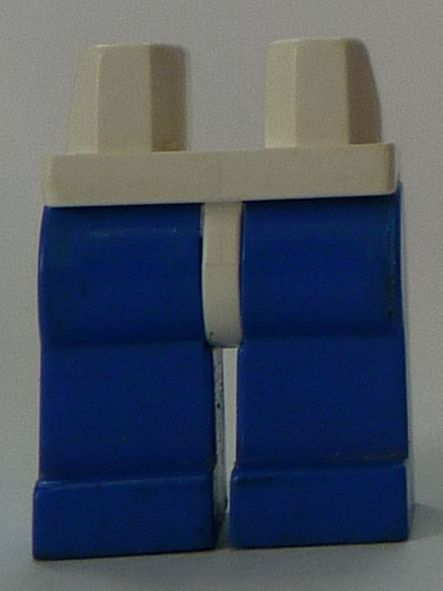
\includegraphics[width=.17\linewidth]{pants-blue} in product 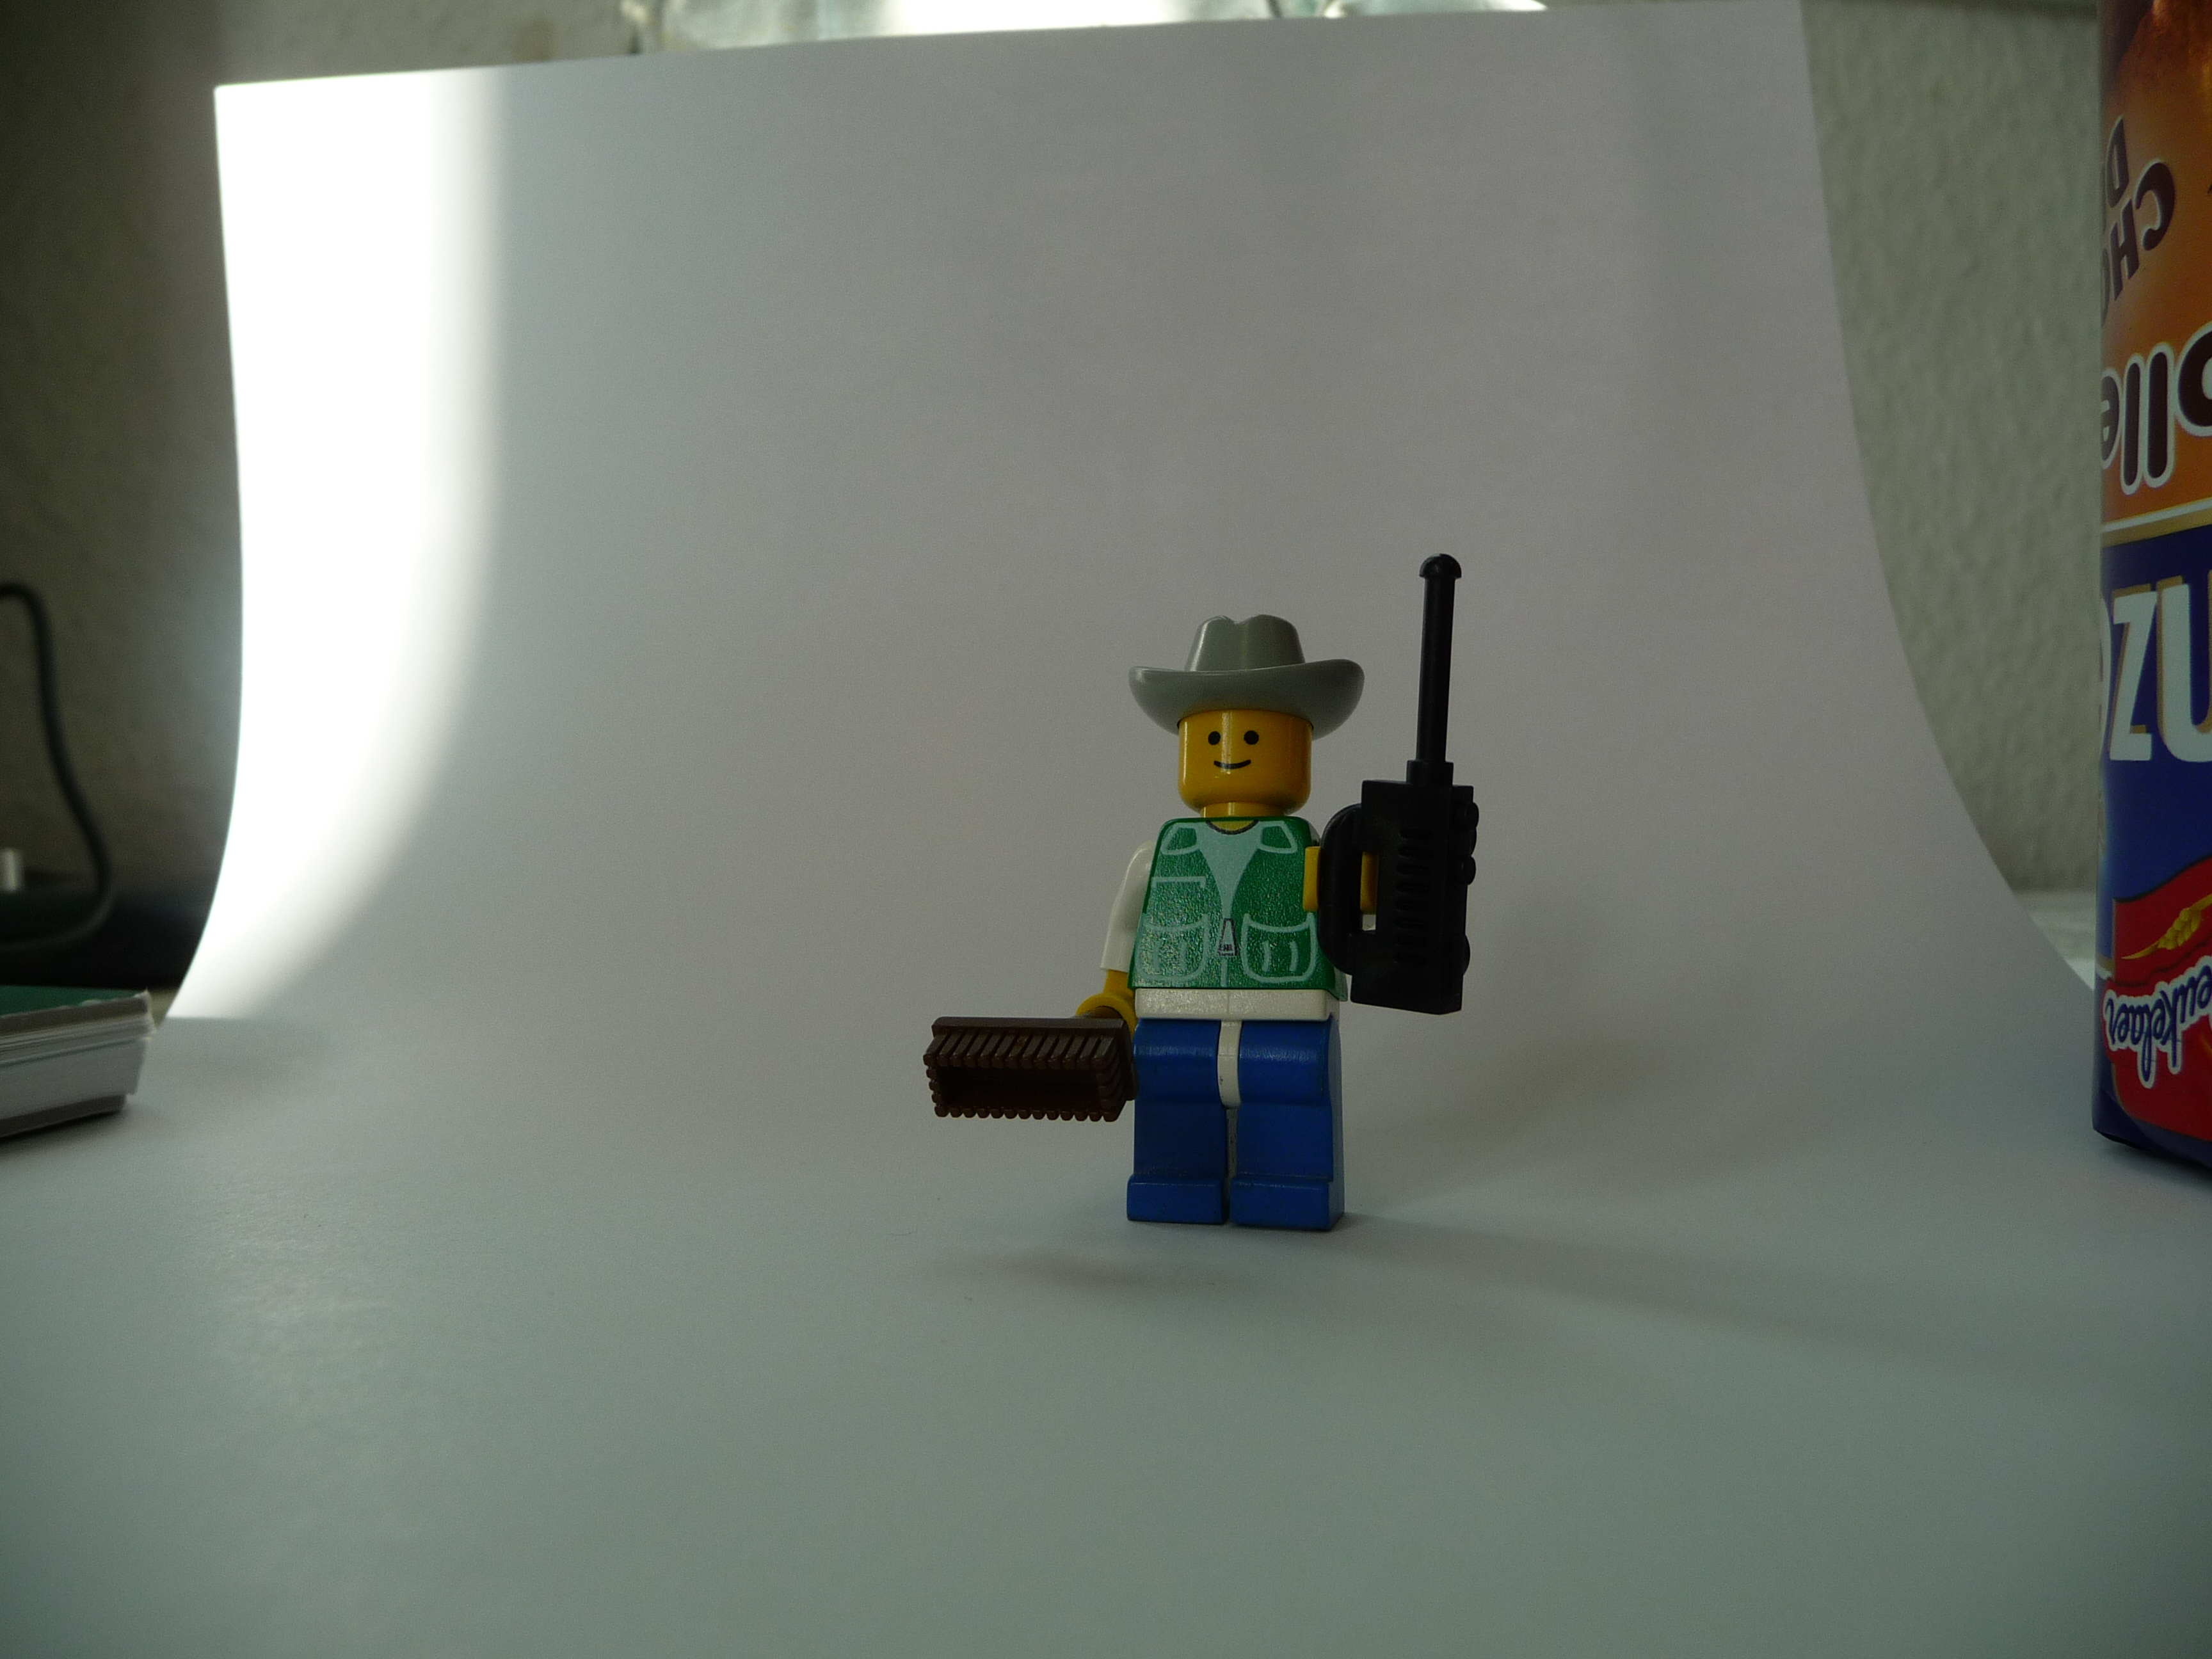
\includegraphics[width=.17\linewidth]{230}
		\end{example}
	\mynextcolumn
		\myexampletight{Feature Traceability with Colored Source Code}{\picDark[width=\linewidth]{feature-traceability}}
	\end{mycolumns}
\end{frame}

\subsection{Automated Generation}
\begin{frame}{\myframetitle}
	\begin{mycolumns}[columns=3,widths={37,7},animation=none]
		\myexampletight{Features}{
			\foreach \animation/\handout/\page in {1-2/0/5,3-4/0/6,5-6/0/7,7-8/0/8,9-10/0/9,11-/1/10} {%
				\only<\animation|handout:\handout>{\includegraphics[width=\linewidth,page=\page,trim=45 0 45 0,clip]{lego}}%
			}%
		}
	\mynextcolumn
		\centering\Huge$\Rightarrow$
	\mynextcolumn
		\myexampletight{Products}{
			\foreach \animation/\handout/\page in {1/0/3,2-3/0/11,4-5/0/12,6-7/0/13,8-9/0/14,10-11/0/15,12-/1/18} {%
				\only<\animation|handout:\handout>{\includegraphics[width=\linewidth,page=\page]{lego}}%
			}%
		}
	\end{mycolumns}
\end{frame}
\begin{frame}{\myframetitle}
	\begin{mycolumns}[widths={45},animation=none]
		\begin{example}{Product Line with Features}
			\only<1-2|handout:0>{
\includegraphics[width=\linewidth]{metaproduct}}%
			\only<3->{
\includegraphics[width=\linewidth]{metaproduct2}}%
		\end{example}
	\mynextcolumn
		\begin{definition}{Goal}
			\begin{itemize}
			\item automatic generation of products
			\item based on a (descriptive) selection of features
			\end{itemize}
		\end{definition}
		\uncover<2->{\begin{note}{Challenges}
			\begin{itemize}
			\item how to map features to source code?
			\item how to combine source code of multiple features?
			\item how to define valid combinations of features?
			\end{itemize}
		\end{note}}
	\end{mycolumns}
\end{frame}

\subsection{Combinatorial Explosion}
\begin{frame}{\myframetitle}
	\begin{mycolumns}[widths={49}]
		\myexampletight{Combinatorial Explosion}{
			\includegraphics[width=\linewidth,page=6]{cit-plots}%
			\small%
			\begin{itemize}
				\item assumption: all combinations of features are valid
				\item 33 features: a unique combination for every human
				\item 320 features: more combinations than atoms in the universe
			\end{itemize}
		}
	\mynextcolumn
		\myexampletight{Industrial Configuration Spaces \mysource{\evaluatingsharpsatsolvers}}{
			\evaluatingsharpsatsolverslink{\includegraphics[width=\linewidth,page=6,trim=50 210 320 440,clip]{2020/2020-VaMoS-Sundermann}}%
			\small%
			\begin{itemize}
				\item in practice: not all combinations of features valid
				\item many industrial product lines too large to specify all valid combinations separately
				\item largest automotive product line has about $1.7 \cdot 10^{1534}$ products
			\end{itemize}
		}
	\end{mycolumns}
\end{frame}
\begin{frame}{\myframetitle}
	\centering\href{https://github.com/SoftVarE-Group/Slides/blob/main/2021/2021-02-10-VaMoS-SharpSATApplications.pdf}{\includegraphics[height=\textheightwithtitle,page=9,trim=60 15 15 5,clip]{2021/2021-02-10-VaMoS-SharpSATApplications}}
\end{frame}

\subsection{Feature Interactions}
\begin{frame}{\myframetitle}
	\begin{mycolumns}
		\only<1-2|handout:0>{\includegraphics[width=\linewidth,page=24]{lego}}%
		\only<3->{\includegraphics[width=\linewidth,page=25]{lego}}%
	\mynextcolumn
		\begin{example}{Example Interaction}
			phone 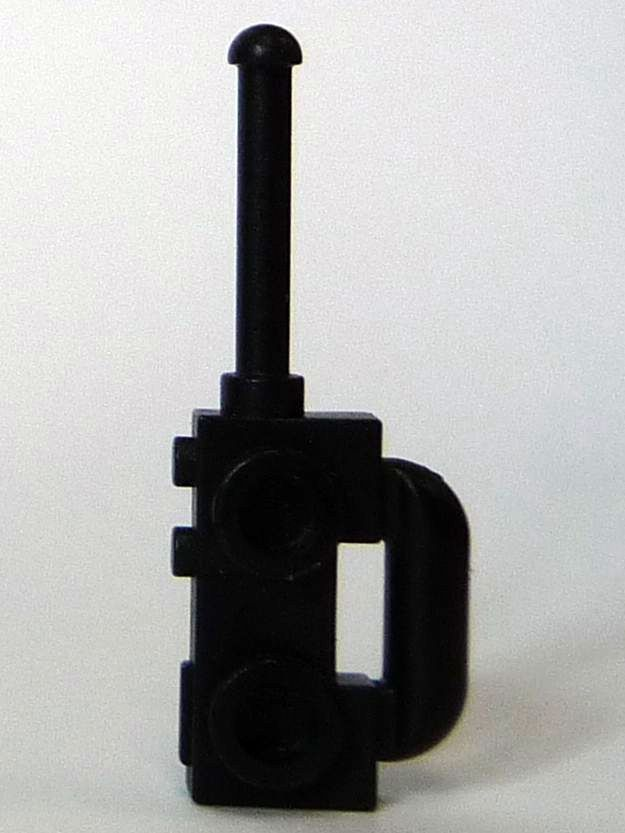
\includegraphics[width=.14\linewidth]{phone} cannot be used with helmet 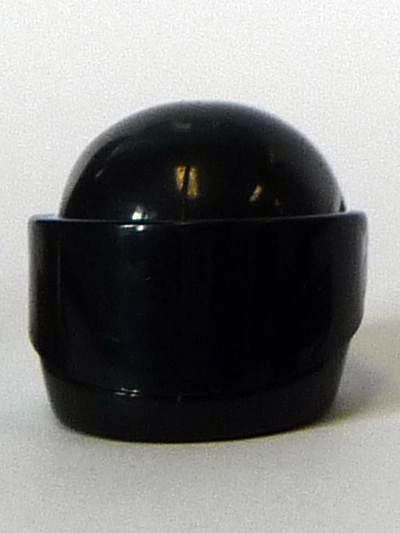
\includegraphics[width=.14\linewidth]{helmet}
		\end{example}
		\uncover<2->{\begin{note}{Challenges}
			\begin{itemize}
			\item interaction typically unknown in advance
			\item interactions occur in some but not all combinations
			\item challenge for quality assurance
			\end{itemize}
		\end{note}}
	\end{mycolumns}
\end{frame}
\begin{frame}{\myframetitle}
	\begin{mycolumns}[columns=3,widths={13,74},animation=none]
	\mynextcolumn
		\myexampletight{Invalid Car Configurations}{\picDark[width=\linewidth]{bmw-series1-confassistant-bluetooth}}
	\mynextcolumn
	\end{mycolumns}
\end{frame}

\subsection{Continuing Change and Growth}
\begin{frame}{\myframetitle}
	\begin{mycolumns}[widths={42}]
		\begin{definition}{Lehman's Laws of Software Evolution (excerpt) \mysource{\lehmanslaws}}
			\begin{itemize}
				\item Continuing Change: systems must be continually adapted to stay satisfactory % E-type systems must be continually adapted else they become progressively less satisfactorv.
				\item Increasing Complexity: complexity increases during evolution unless work is done to maintain or reduce it % As an E-type system evolves its complexity increases unless work is done to maintain or reduce it.
				%\item Self Regulation: %E-type system evolution process is self regulating with distribution of product and process measures close to normal.
				%\item Conservation of Organizational Stability (invariant work rate): %The average effective global activity rate in an evolving E-type system is invariant over product lifetime.
				%\item Conservation of Familiarity: satisfactory evolution excludes excessive growth %As an E-type system evolves all associated with it, developers, sales personnel, users, for example, must maintain mastery of its content and behaviour to achieve satisfactory evolution. Excessive growth diminishes that mastery. Hence the average incremental growth remains invariant as the system evolves.
				\item Continuing Growth: functionality must be continually increased to maintain user satisfaction %The functional content of E-type systems must be continually increased to maintain user satisfaction over their lifetime.
				\item Declining Quality: quality will decline unless rigorously maintained and adapted to operational environment changes %The quality of E-type systems will appear to be declining unless they are rigorously maintained and adapted to operational environment changes.
				%\item Feedback System: %E-type evolution processes constitute multi-level, multi-loop, multi-agent feedback systems and must be treated as such to achieve significant improvement over any reasonable base.
			\end{itemize}
		\end{definition}
	\mynextcolumn
		\begin{note}{Essence of the Laws}
			\begin{itemize}
				\item software that is used will be modified
				\item when modified, its complexity will increase (unless one does actively work against it)
			\end{itemize}
		\end{note}
		\begin{example}{Consequences for Product Lines}
			\begin{itemize}
				\item number of features and size of implementation increases over time
				\item discussed challenges increase over time
					\begin{itemize}
						\item more software clones
						\item harder to trace features
						\item automated generation more urgent
						\item increasing combinatorial explosion
						\item more feature interactions
					\end{itemize}
			\end{itemize}
		\end{example}
	\end{mycolumns}
\end{frame}

\begin{frame}{Evolution of the Linux Kernel}
	\begin{mycolumns}
		\begin{example}{}
			\begin{itemize}
				\item about $60,000$ commits per year
				\item in peak weeks: new commit every 5 minutes
				\item in average weeks: every 9 minutes
			\end{itemize}
		\end{example}
	\mynextcolumn
		\vspace{-\textheightoftitle}
		\picDark[width=\linewidth,trim=100 70 110 80,clip]{linux-stack-plot}
	\end{mycolumns}
	\twodimensionalanalysislink{\includegraphics[width=.8\linewidth,page=1,trim=80 420 80 260,clip]{2019/2019-VariVolution-Thuem}}
\end{frame}

\begin{frame}{Evolution of the Linux Kernel}
	\begin{mycolumns}
		\myexampletight{Size of the Code Base}{
			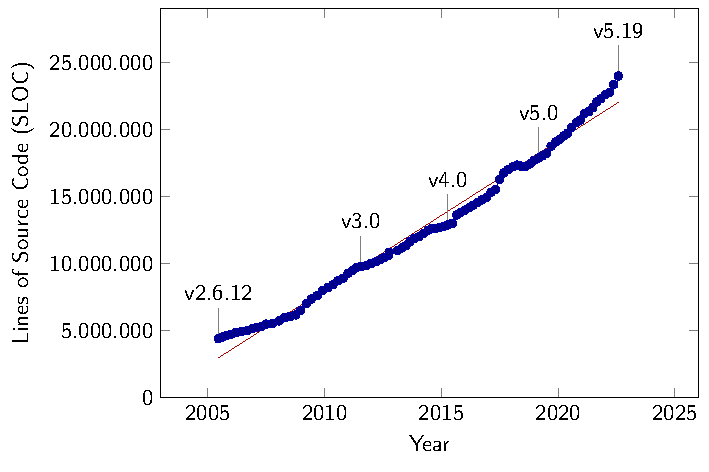
\includegraphics[width=\linewidth,page=1]{linux-plots}%
			\begin{itemize}
				\item from 4 to 24 millions in 17 years
				\item about one million LOC added every year
				\item about 3,000 LOC per day
			\end{itemize}
		}
	\mynextcolumn
		\myexampletight{Number of Features}{
			\includegraphics[width=\linewidth,page=2]{linux-plots}%
			\begin{itemize}
				\item about 800 new features every year
				\item about 15 new features every week
				\item in 2018 four times more features than in 2005
			\end{itemize}
		}
	\end{mycolumns}
\end{frame}

\begin{frame}{Evolution of the Linux Kernel}
	\begin{mycolumns}
		\myexampletight{Number of Products}{
			\includegraphics[width=\linewidth,page=3]{linux-plots}%
			\begin{itemize}
				\item number of products grows by factor 100.000 each month
				\item the current kernel is likely to have more than $10^{1500}$ products
			\end{itemize}
		}
	\mynextcolumn
		\myexampletight{Time to Count Products}{
			\includegraphics[width=\linewidth,page=4]{linux-plots}%
			\begin{itemize}
				\item most kernel versions before 2006 can be computed within 1 minute
				\item most kernel versions after 2006 cannot be computed within 1 hour
			\end{itemize}
		}
	\end{mycolumns}
\end{frame}

% costs: development, investment, maintenance, logistic, production
% customer needs?



\lessonslearned{
	\item why are product lines challenging?
	\item selected challenges:
		\begin{enumerate}
		\item software clones
		\item feature traceability
		\item automated generation
		\item combinatorial explosion
		\item feature interactions
		\item continuous growth
		\end{enumerate}
}{
	\item[] see later lectures
}{
	\begin{itemize}
		\item Form groups of 2--3 students
		\item Explain 2--3 of the six challenges to your colleagues
		\item Can you find own examples for these challenges?
	\end{itemize}
}

\sectionend

\section{Course Organization}

\subsection{What You Should Know}

\begin{frame}{\myframetitle{}}
	\begin{mycolumns}
		\mynote{Fundamentals of Software Engineering}{
			\begin{itemize}
				\item development processes
				\item object-oriented programming
				\item design patterns
				\item UML class diagrams
				\item modularity
			\end{itemize}
			\ifuniversity{magdeburg}{$\Rightarrow$ \emph{Software Engineering}}
		}
	\mynextcolumn
		\mynote{Fundamentals of Theoretical Computer Science}{
			\begin{itemize}
				\item set theory
				\item propositional logic
				\item complexity theory
			\end{itemize}
			\ifuniversity{magdeburg}{
				$\Rightarrow$ \emph{Logik}\\
				$\Rightarrow$ \emph{Grundlagen der Theoretischen Informatik I}
			}
		}

		\mynote{Exercise}{
			solid programming skills in Java

			\ifuniversity{magdeburg}{
				$\Rightarrow$ \emph{Einführung in die Informatik}\\
				$\Rightarrow$ \emph{Algorithmen und Datenstrukturen}
			}
		}
	\end{mycolumns}
\end{frame}

\subsection{What You Will Learn}

\begin{frame}{\myframetitle{}}
	\lectureseriesoverview
\end{frame}

\subsection{What You Might Need}

\begin{frame}{\myframetitle{}}
	\begin{mycolumns}
		\myexampletight{Recommended Literature for Lecture \& Exercise}{
			\centering
			\parbox{0.49\linewidth}{
				\centering
				\pic[width=\linewidth]{cover-fospl}
				\emph{theory-focused}
			}
			\parbox{0.475\linewidth}{
				\centering
				\pic[width=\linewidth]{cover-featureide}
				\emph{practice-oriented}
			}
		}
	\mynextcolumn
		\myexampletight{Recommended Tool Support for the Exercise}{
			\centering
			\pic[width=\linewidth]{featureide-feature-model-editor}\\[.5ex]
			\pic[width=0.25\linewidth]{featureide-logo}
		}
	\end{mycolumns}
\end{frame}

\subsection{Credit for the Slides}

\begin{frame}{\myframetitle{}}
	\vspace{-10mm}\hfill\href{https://github.com/SoftVarE-Group/Course-on-Software-Product-Lines}{
\includegraphics[scale=.5]{cc-by-sa}}\vspace{2mm}
	\begin{mycolumns}[columns=3,animation=none]
		\mynote{Thomas Thüm}{
			\centering
			\href{https://www.uni-ulm.de/en/in/sp/team/thuem/}{\adjincludegraphics[height=.45\textheight,trim={.125\width} 0 {.125\width} 0,clip]{thomas-thuem}}

			\small Professor at University of Ulm

			software engineering

			FeatureIDE team leader
		}
	\mynextcolumn
		\mynote{Timo Kehrer}{
			\centering
			\href{https://seg.inf.unibe.ch/people/timo/}{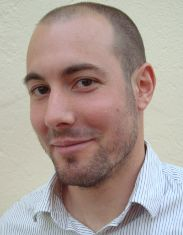
\includegraphics[height=.45\textheight]{timo-kehrer}}

			\small Professor at University of Bern

			software engineering

			~
		}
	\mynextcolumn
		\mynote{Elias Kuiter}{
			\centering
			\href{https://www.dbse.ovgu.de/en/Staff/Elias+Kuiter.html}{
\includegraphics[height=.45\textheight]{elias-kuiter}}

			\small PhD student in Magdeburg

			feature-model analysis

			FeatureIDE core developer
		}
	\end{mycolumns}
\end{frame}
\inputifuniversity{content/01c-course}

\lessonslearned{
	\item focus: how to implement features
	\item focus: how to model valid combinations
	\item focus: how to do quality assurance
	\item prerequisites, course overview, formalities
}{
	\item \fospl
 	\item \featureide
}{
	\begin{itemize}
		\item Ask questions on the course organization!
		\item Form teams for the practical tasks.
	\end{itemize}
}

\mode<beamer>{
	\begin{frame}{\inserttitle}
		\lectureseriesoverview
	\end{frame}

	\contentoverview
}


\end{document}
